\begin{exercice*}
    Le triangle $ABC$ est une réduction du triangle $EDF$.

    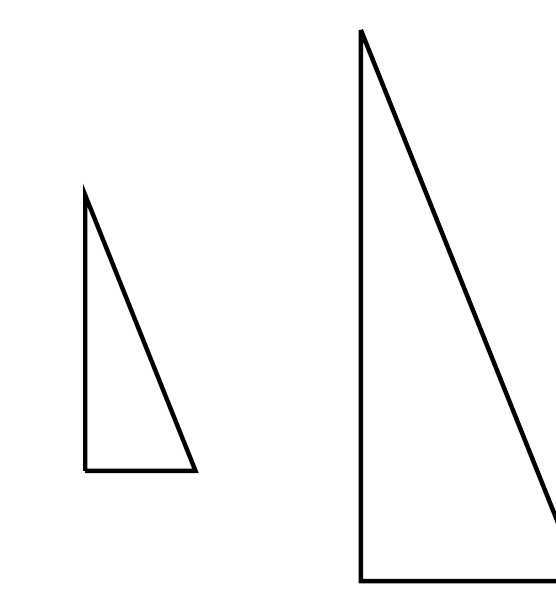
\begin{tikzpicture}[scale = 0.7]
            %     \draw[help lines, color=black!70, dashed] (0,0) grid (11,11);                            
            \coordinate (A) at (1,3);
            \coordinate (B) at (1,8);
            \coordinate (C) at (3,3);
            \coordinate (D) at (6,11);
            \coordinate (E) at (6,1);
            \coordinate (F) at (10,1);                                
            \tkzDrawSegment[style=red, dashed,dim={$\Lg{5}$,15pt,midway,font=\normalsize,sloped}](A,B)        
            \tkzDrawSegment[style=red, dashed,dim={$\Lg{15}$,15pt,midway,font=\normalsize,sloped}](E,D)        
            \tkzDrawSegment[style=red, dashed,dim={$\Lg{6}$,-15pt,midway,font=\normalsize,sloped}](E,F)
            \draw[ultra thick] (A)--(B)--(C)--(A);
            \draw[ultra thick] (D)--(E)--(F)--(D);
            \tkzLabelPoints[above](B,D);
            \tkzLabelPoints[below](A,C);
            \tkzLabelPoints[below left](E);
            \tkzLabelPoints[below right](F);
    \end{tikzpicture}

    Recopier et compléter.
    \begin{enumerate}
        \item On sait que le triangle $ABC$ est une \makebox[1cm]{\dotfill} du triangle $EDF$.
        Donc leurs \makebox[1cm]{\dotfill} sont proportionnelles.
        On en déduit le rapport $k$ de réduction :

        $k=\dfrac{AB}{ED}=\dfrac{\makebox[1cm]{\dotfill}}{\makebox[1cm]{\dotfill}}=\dfrac{\makebox[1cm]{\dotfill}}{\makebox[1cm]{\dotfill}}$
        
        \smallskip
        \item $[AC]$ est une \makebox[1cm]{\dotfill} de rapport $\dfrac{\makebox[1cm]{\dotfill}}{\makebox[1cm]{\dotfill}}$ de $[EF]$, donc 
        $AC=\dfrac{\makebox[1cm]{\dotfill}}{\makebox[1cm]{\dotfill}}\times EF=\makebox[1cm]{\dotfill} \Lg{}$
    \end{enumerate}
\end{exercice*}
\begin{corrige}
    %\setcounter{partie}{0} % Pour s'assurer que le compteur de \partie est à zéro dans les corrigés
    \phantom{rrr}  

    \begin{minipage}{0.3\linewidth}
        Le triangle $ABC$ est une réduction du triangle $EDF$.

        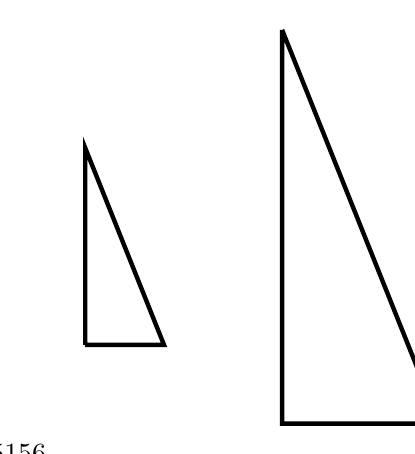
\begin{tikzpicture}[scale = 0.5]
                %     \draw[help lines, color=black!70, dashed] (0,0) grid (11,11);                            
                \coordinate (A) at (1,3);
                \coordinate (B) at (1,8);
                \coordinate (C) at (3,3);
                \coordinate (D) at (6,11);
                \coordinate (E) at (6,1);
                \coordinate (F) at (10,1);                                
                \tkzDrawSegment[style=red, dashed,dim={$\Lg{5}$,15pt,midway,font=\normalsize,sloped}](A,B)        
                \tkzDrawSegment[style=red, dashed,dim={$\Lg{15}$,15pt,midway,font=\normalsize,sloped}](E,D)        
                \tkzDrawSegment[style=red, dashed,dim={$\Lg{6}$,-15pt,midway,font=\normalsize,sloped}](E,F)
                \draw[ultra thick] (A)--(B)--(C)--(A);
                \draw[ultra thick] (D)--(E)--(F)--(D);
                \tkzLabelPoints[above](B,D);
                \tkzLabelPoints[below](A,C);
                \tkzLabelPoints[below left](E);
                \tkzLabelPoints[below right](F);
        \end{tikzpicture}
    \end{minipage}
    \hfill
    \begin{minipage}{0.55\linewidth}
        Recopier et compléter. 

        \begin{enumerate}
            \item On sait que le triangle $ABC$ est une {\color{red}réduction} du triangle $EDF$.
            Donc leurs {\color{red}longueurs} sont proportionnelles.
            On en déduit le rapport $k$ de réduction :

            $k=\dfrac{AB}{ED}=\dfrac{{\color{red}5}}{{\color{red}15}}=\dfrac{{\color{red}1}}{{\color{red}3}}$
            
            \smallskip
            \item $[AC]$ est une {\color{red}réduction} de rapport $\dfrac{{\color{red}1}}{{\color{red}3}}$ de $[EF]$,
            
            donc $AC=\dfrac{{\color{red}1}}{{\color{red}3}}\times EF={\color{red}2~} \Lg{}$
        \end{enumerate}
    \end{minipage}
\end{corrige}